% \documentclass[table]{beamer}
\documentclass[table,handout]{beamer}
\setbeameroption{show notes}
% \setbeameroption{hide notes}
% \setbeameroption{show only notes}
\usepackage{varwidth}

\newif\ifhide
\newif\ifpost
\newif\ifhideclicker

% \hidetrue
% \hideclickertrue
% \posttrue

\newcommand{\whiteout}[1]{\textcolor{white}{#1}}
% \newcommand{\whiteoutbox}[1]{\fcolorbox{white}{white}{\parbox{\dimexpr \linewidth-2\fboxsep-2\fboxrule}{\whiteout{#1}}}}
% \newcommand{\notebox}[1]{\fcolorbox{blue}{white}{\parbox{\dimexpr \linewidth-2\fboxsep-2\fboxrule}{#1}}}
\newcommand{\whiteoutbox}[1]{\fcolorbox{white}{white}{\parbox{\linewidth}{\whiteout{#1}}}}
\newcommand{\notebox}[1]{\fcolorbox{blue}{white}{\parbox{\linewidth}{#1}}}
\newcommand{\blankbox}[1]{\phantom{\varwidth{\linewidth}\whiteoutbox{#1}\endvarwidth}}
\newcommand{\blank}[1]{\phantom{\varwidth{\linewidth}#1\endvarwidth}}

\ifhide%
    \newcommand{\hmask}[1]{\blank{#1}}%
\else%
    \newcommand{\hmask}[1]{#1}%
\fi

\ifhide%
    \newcommand{\wout}[1]{\whiteout{#1}}%
\else%
    \newcommand{\wout}[1]{#1}%
\fi

\ifhide%
    \newcommand{\hignore}[1]{}%
\else%
    \newcommand{\hignore}[1]{#1}%
\fi

\ifpost%
    \newcommand{\nopost}[1]{}%
\else%
    \newcommand{\nopost}[1]{#1}%
\fi

\ifhideclicker%
    \newcommand{\clickerslide}[1]{\stepcounter{clickerQuestionCounter}%
        \begin{frame}[t]
            \textcolor{blue}{Q \arabic{clickerQuestionCounter}:}
        \end{frame}}
\else%
    \newcommand{\clickerslide}[1]{#1}%
\fi

\ifhide%
    \newcommand{\hidebox}[1]{\blank{#1}}%
\else%
    \newcommand{\hidebox}[1]{\notebox{#1}}%
\fi

\ifhide%
    \newcommand{\wbox}[1]{\whiteoutbox{#1}}%
\else%
    \newcommand{\wbox}[1]{\notebox{#1}}%
\fi

\ifhide%
    \newcommand{\nbox}[1]{\blankbox{#1}}%
\else%
    \newcommand{\nbox}[1]{\notebox{#1}}%
\fi

\ifhideclicker%
    \newcommand{\clickeranswer}[1]{#1}%
\else%
    \ifhide%
        \newcommand{\clickeranswer}[1]{#1}%
    \else%
        \newcommand{\clickeranswer}[1]{\textbf{\textcolor{blue}{#1}}}%
    \fi
\fi

\usepackage{beamerthemesplit}
% \usetheme{boxes}
\usetheme{Malmoe}
\usecolortheme{seahorse}
% \usecolortheme{seagull}
\usepackage{ifthen}
\usepackage{xspace}
\usepackage{multirow}
\usepackage{multicol}
\usepackage{booktabs}
\usepackage{xcolor}
\usepackage{wasysym}
\usepackage{comment}
\usepackage{hyperref}
\hypersetup{pdfborder={0 0 0}, colorlinks=true, urlcolor=blue, linkcolor=blue, citecolor=blue}
\usepackage{changepage}
\usepackage[compatibility=false]{caption}
\captionsetup[figure]{font=scriptsize, labelformat=empty, textformat=simple, justification=centering, skip=2pt}
\usepackage{tikz}
\usetikzlibrary{trees,calc,backgrounds}

\usepackage[bibstyle=joaks-slides,maxcitenames=3,mincitenames=1,backend=biber]{biblatex}

\newrobustcmd*{\shortfullcite}{\AtNextCite{\renewbibmacro{title}{}\renewbibmacro{in:}{}\renewbibmacro{number}{}}\fullcite}

\newrobustcmd*{\footlessfullcite}{\AtNextCite{\renewbibmacro{title}{}\renewbibmacro{in:}{}}\footfullcite}

% Make all footnotes smaller
% \renewcommand{\footnotesize}{\scriptsize}

\definecolor{myGray}{gray}{0.9}
\colorlet{rowred}{red!30!white}

\setbeamertemplate{blocks}[rounded][shadow=true]

\setbeamercolor{defaultcolor}{bg=structure!30!normal text.bg,fg=black}
\setbeamercolor{block body}{bg=structure!30!normal text.bg,fg=black}
\setbeamercolor{block title}{bg=structure!50!normal text.bg,fg=black}

\newenvironment<>{varblock}[2][\textwidth]{%
  \setlength{\textwidth}{#1}
  \begin{actionenv}#3%
    \def\insertblocktitle{#2}%
    \par%
    \usebeamertemplate{block begin}}
  {\par%
    \usebeamertemplate{block end}%
  \end{actionenv}}

\newenvironment{displaybox}[1][\textwidth]
{
    \centerline\bgroup\hfill
    \begin{beamerboxesrounded}[lower=defaultcolor,shadow=true,width=#1]{}
}
{
    \end{beamerboxesrounded}\hfill\egroup
}

\newenvironment{onlinebox}[1][4cm]
{
    \newbox\mybox
    \newdimen\myboxht
    \setbox\mybox\hbox\bgroup%
        \begin{beamerboxesrounded}[lower=defaultcolor,shadow=true,width=#1]{}
    \centering
}
{
    \end{beamerboxesrounded}\egroup
    \myboxht\ht\mybox
    \raisebox{-0.25\myboxht}{\usebox\mybox}\hspace{2pt}
}

\newenvironment{mydescription}{
    \begin{description}
        \setlength{\leftskip}{-1.5cm}}
    {\end{description}}

\newenvironment{myitemize}{
    \begin{itemize}
        \setlength{\leftskip}{-.3cm}}
    {\end{itemize}}

% footnote without a marker
\newcommand\barefootnote[1]{%
  \begingroup
  \renewcommand\thefootnote{}\footnote{#1}%
  \addtocounter{footnote}{-1}%
  \endgroup
}

% define formatting for footer
\newcommand{\myfootline}{%
    {\it
    \insertshorttitle
    \hspace*{\fill} 
    \insertshortauthor, \insertshortinstitute
    % \ifx\insertsubtitle\@empty\else, \insertshortsubtitle\fi
    \hspace*{\fill}
    \insertframenumber/\inserttotalframenumber}}

% set up footer
\setbeamertemplate{footline}{%
    \usebeamerfont{structure}
    \begin{beamercolorbox}[wd=\paperwidth,ht=2.25ex,dp=1ex]{frametitle}%
        % \Tiny\hspace*{4mm}\myfootline\hspace{4mm}
        \tiny\hspace*{4mm}\myfootline\hspace{4mm}
    \end{beamercolorbox}}

% remove navigation bar
\beamertemplatenavigationsymbolsempty

\makeatletter
    \newenvironment{noheadline}{
        \setbeamertemplate{headline}[default]
        \def\beamer@entrycode{\vspace*{-\headheight}}
    }{}
\makeatother

\newcounter{clickerQuestionCounter}
\ifhideclicker%
\newenvironment{clickerquestion}
{ \stepcounter{clickerQuestionCounter}
  \begin{enumerate}[Q \arabic{clickerQuestionCounter}:]\color{white} }
{ \end{enumerate} }
\else%
\newenvironment{clickerquestion}
{ \stepcounter{clickerQuestionCounter}
  \begin{enumerate}[Q \arabic{clickerQuestionCounter}:] }
{ \end{enumerate} }
\fi

\ifhideclicker%
\newenvironment{clickeroptions}
{ \begin{enumerate}[\begingroup\color{white} 1)\endgroup]\color{white} }
{ \end{enumerate} }
\else%
\newenvironment{clickeroptions}
{ \begin{enumerate}[\begingroup\color{red} 1)\endgroup] }
{ \end{enumerate} }
\fi


\tikzstyle{centered} = [align=center, text centered, font=\sffamily\bfseries]
\tikzstyle{skip} = [centered, inner sep=0pt, fill]
\tikzstyle{empty} = [centered, inner sep=0pt]
\tikzstyle{inode} = [centered, circle, minimum width=4pt, fill=black, inner sep=0pt]
\tikzstyle{tnode} = [centered, circle, inner sep=1pt]
\tikzset{
  % edge styles
  level distance=10mm,
  mate/.style={edge from parent/.style={draw,distance=3pt}},
  mleft/.style={grow=left, level distance=10mm, edge from parent path={(\tikzparentnode.west)--(\tikzchildnode.east)}},
  mright/.style={grow=right, level distance=10mm, edge from parent path={(\tikzparentnode.east)--(\tikzchildnode.west)}},
  % node styles
  male/.style={rectangle,minimum size=4mm,fill=gray!80},
  female/.style={circle,minimum size=4mm,fill=gray!80},
  amale/.style={male,fill=red},
  afemale/.style={female,fill=red},
}

\newcommand{\highlight}[1]{\textcolor{violet}{\textit{\textbf{#1}}}}
\newcommand{\super}[1]{\ensuremath{^{\textrm{\sffamily #1}}}}
\newcommand{\sub}[1]{\ensuremath{_{\textrm{\sffamily #1}}}}
\newcommand{\dC}{\ensuremath{^\circ{\textrm{C}}}}
\newcommand{\tb}{\hspace{2em}}
\providecommand{\e}[1]{\ensuremath{\times 10^{#1}}}
\newcommand{\myHangIndent}{\hangindent=5mm}

\newcommand{\spp}[1]{\textit{#1}}

\newcommand\mybullet{\leavevmode%
\usebeamertemplate{itemize item}\hspace{.5em}}

\makeatletter
\newcommand*{\rom}[1]{\expandafter\@slowromancap\romannumeral #1@}
\makeatother

\newcommand{\blankslide}{{\setbeamercolor{background canvas}{bg=black}
\setbeamercolor{whitetext}{fg=white}
\begin{frame}<handout:0>[plain]
\end{frame}}}

\newcommand{\whiteslide}{
\begin{frame}<handout:0>[plain]
\end{frame}}

\newcommand{\f}[1]{\ensuremath{F_{#1}}}
\newcommand{\x}[1]{X\ensuremath{^{#1}}}
\newcommand{\y}[1]{Y\ensuremath{^{#1}}}

% Population growth macros
\newcommand{\popsize}[1]{\ensuremath{N_{#1}}}
\newcommand{\popgrowthratediscrete}[1]{\ensuremath{\lambda_{#1}}}
\newcommand{\popgrowthrate}[1]{\ensuremath{r_{#1}}}
\newcommand{\ptime}{\ensuremath{t}\xspace}

\tikzset{hide on/.code={\only<#1>{\color{white}}}}
\tikzset{
    invisible/.style={opacity=0},
    visible on/.style={alt={#1{}{invisible}}},
    alt/.code args={<#1>#2#3}{%
        \alt<#1>{\pgfkeysalso{#2}}{\pgfkeysalso{#3}}
        % \pgfkeysalso doesn't change the path
    },
}

% \bibliography{../bib/references}
\bibliography{references}
\author[J.\ Oaks]{
    %Jamie R.\ Oaks\inst{1}
    Jamie R.\ Oaks
}
\institute[BIOL 180]{
    \inst{}%
        BIOL 180: Introductory Biology
}



\title[Intro \& Experimental Design]{Course Introduction \& Experimental Design}
% \date{\today}
\date{March 30, 2015}

\begin{document}

\begin{noheadline}
\maketitle
\end{noheadline}

% \nopost{
% \begin{noheadline}
% \begin{frame}[c]
%     \vspace{-3mm}
%     \begin{center} 
%         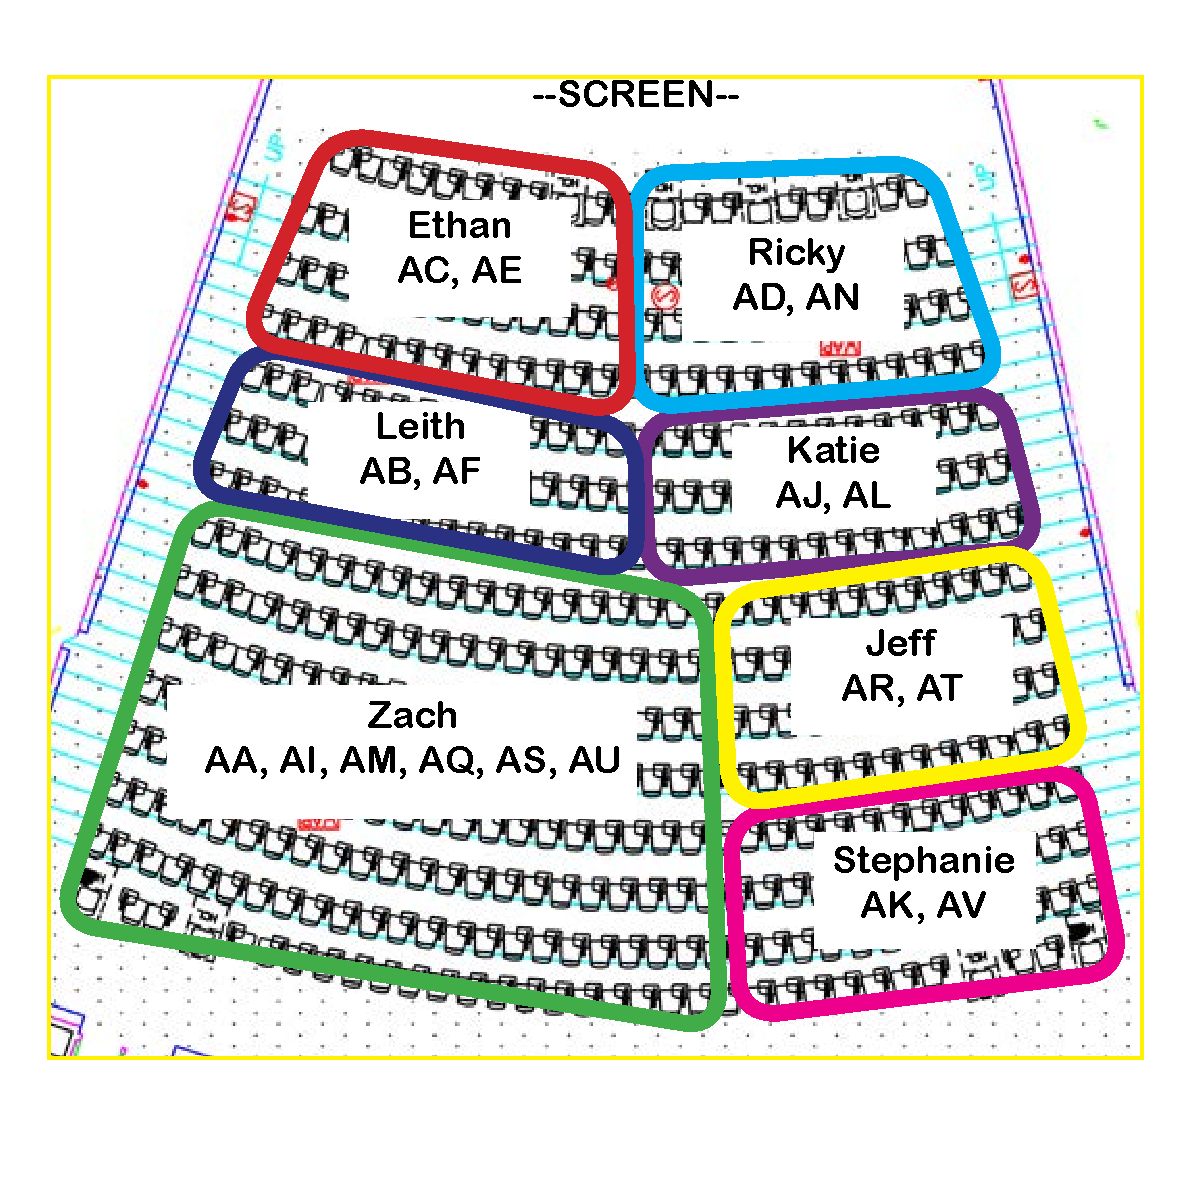
\includegraphics[height=1.1\textheight]{../images/seating-chart.pdf}
%     \end{center}
% \end{frame}
% \end{noheadline}
% }

% The people
\begin{noheadline}
\begin{frame}
\frametitle{Welcome to Biology 180!}

    \begin{table}%[htbp]
        \centering
        \begin{tabular}{ l l }
            \textbf{Instructor} & \\
            Jamie Oaks & \href{mailto:joaks1@uw.edu}{joaks1@uw.edu} \\[1.5ex]
            \textbf{Staff} & \\
            John Parks, Course Coordinator & \href{mailto:jwparks@uw.edu}{jwparks@uw.edu} \\
            Celese Spencer, Field Trips & \href{mailto:celese@uw.edu}{celese@uw.edu} \\[1.5ex]
            \textbf{Teaching Assistants} \\
        \end{tabular}
    \end{table}

\end{frame}
\end{noheadline}

\begin{noheadline}
\begin{frame}
    \begin{adjustwidth}{-2em}{-2em}
\includegraphics<1| handout:0>[page=1,width=\paperwidth]{./johns-slides.pdf}
\includegraphics<2| handout:0>[page=2,width=\paperwidth]{./johns-slides.pdf}
\includegraphics<3| handout:0>[page=3,width=\paperwidth]{./johns-slides.pdf}
\includegraphics<4| handout:1>[page=4,width=\paperwidth]{./johns-slides.pdf}
\includegraphics<5| handout:0>[page=5,width=\paperwidth]{./johns-slides.pdf}
\includegraphics<6| handout:2>[page=6,width=\paperwidth]{./johns-slides.pdf}
\includegraphics<7| handout:0>[page=7,width=\paperwidth]{./johns-slides.pdf}
\includegraphics<8| handout:0>[page=8,width=\paperwidth]{./johns-slides.pdf}
\includegraphics<9| handout:3>[page=9,width=\paperwidth]{./johns-slides.pdf}
    \end{adjustwidth}
\end{frame}
\end{noheadline}

\blankslide

\begin{noheadline}
\begin{frame}
\frametitle{Welcome to Biology 180!}
\tableofcontents[subsectionstyle=hide]
\end{frame}
\end{noheadline}

\section{What are the course goals?}

\begin{noheadline}
\begin{frame}[t]
    \frametitle{What are the course goals?}

    \vspace{-5mm}
    \begin{center}
    \begin{tikzpicture}
        \node[anchor=south west,inner sep=0] (image) at (0,0) {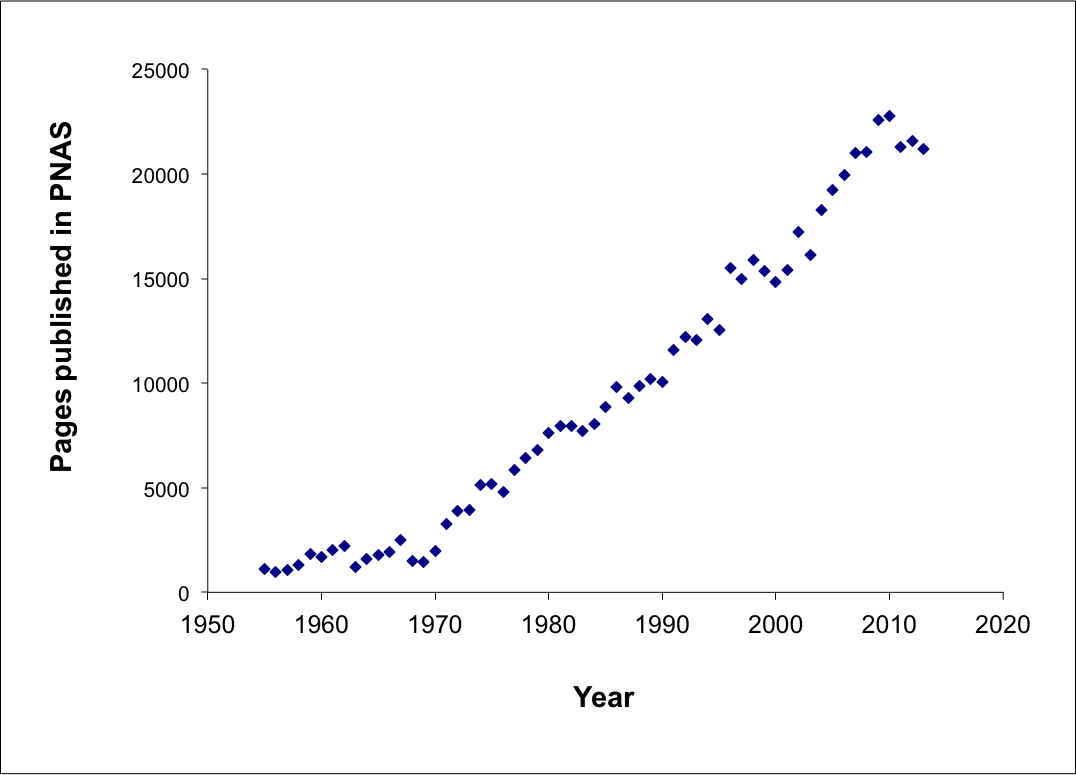
\includegraphics[width=0.95\textwidth]{pnas-pages.png}};
        \begin{scope}[x={(image.south east)},y={(image.north west)}]
            % \draw[red,ultra thick,rounded corners] (0.62,0.65) rectangle (0.78,0.75);
            \onslide<2->{\draw[->,red,ultra thick] (0.52, 0.52) -- (0.52, 0.46);}
            \onslide<3->{\draw[->,red,ultra thick] (0.71, 0.72) -- (0.71, 0.66);}
            \onslide<4->{\draw[->,red,ultra thick] (0.785, 0.85) -- (0.785, 0.79);}
        \end{scope}
    \end{tikzpicture}
    \end{center}

    \vspace{-3mm}
    \uncover<5->{\textbf{What conclusions can you draw from this graph?} \\}
\end{frame}
\end{noheadline}

\begin{noheadline}
\begin{frame}
    \begin{adjustwidth}{-2em}{-2em}
    \vspace{-2cm}
\includegraphics<1| handout:0>[page=28,width=\paperwidth]{./adams-slides.pdf}
\includegraphics<2| handout:0>[page=29,width=\paperwidth]{./adams-slides.pdf}
\includegraphics<3| handout:0>[page=30,width=\paperwidth]{./adams-slides.pdf}
\includegraphics<4| handout:0>[page=31,width=\paperwidth]{./adams-slides.pdf}
\includegraphics<5| handout:0>[page=32,width=\paperwidth]{./adams-slides.pdf}
\includegraphics<6| handout:0>[page=33,width=\paperwidth]{./adams-slides.pdf}
\includegraphics<7| handout:0>[page=34,width=\paperwidth]{./adams-slides.pdf}
\includegraphics<8| handout:0>[page=35,width=\paperwidth]{./adams-slides.pdf}
\includegraphics<9| handout:1>[page=36,width=\paperwidth]{./adams-slides.pdf}
    \end{adjustwidth}
\end{frame}
\end{noheadline}


\begin{noheadline}
\begin{frame}
    \frametitle{What are the course goals?}
    \begin{adjustwidth}{-1em}{-1em}
    \begin{center}
        \textbf{Our job: Prepare you to succeed in Biology 200, upper level
            courses \ldots and possibly a career related to biology.} \\

        \vspace{5mm}
        \uncover<2->{Criteria for Medical School Recommendations:}
    \end{center}
    \end{adjustwidth}

    \begin{adjustwidth}{-2em}{-2em}
    \begin{multicols}{2}
        \begin{itemize}
                \small
            \item<3-> \highlight{Motivation} for training in research
            \item<4-> Intellectual potential \& \highlight{curiosity}
            \item<5-> Ability to \highlight{analyze/problem-solve}
            \item<6-> \highlight{Creativity} and imagination
            \item<7-> \highlight{Oral} communication skills
            \item<8-> \highlight{Written} communication skills
            \item<9-> Ability to \highlight{work with others}
            \item<10-> \highlight{Maturity}
            \item<11-> \highlight{Emotional stability}
            \item<12-> Industrious \& \highlight{persistent}
            \item<13-> Planning \& \highlight{organizational skills}
            \item<14-> Ethics \& \highlight{integrity}
        \end{itemize}
    \end{multicols}

    \begin{uncoverenv}<15->
    \begin{center}
        \textbf{\#1 goal: Teach you how to think like a biologist.}
    \end{center}
    \end{uncoverenv}
    \end{adjustwidth}
\end{frame}
\end{noheadline}


\section{How does this course work?}

% THERE WILL BE A SEATING CHART; WE WILL E-MAIL TO YOU AFTER LECTURE TODAY

\begin{noheadline}
\begin{frame}
    \frametitle{How does this class work?}

    \begin{adjustwidth}{-1.5em}{-1em}
    \begin{columns}

        \column{0.4\linewidth}

        \begin{itemize}
            \item<1-> Cell phones are not allowed in Bio 180
            \item<2-> Why?
            \begin{itemize}
                \item<3-> Professional development
                \item<4-> Student performance
            \end{itemize}
        \end{itemize}

        \column{0.6\linewidth}

        \begin{uncoverenv}<4->
        \begin{figure}
            \begin{center}
            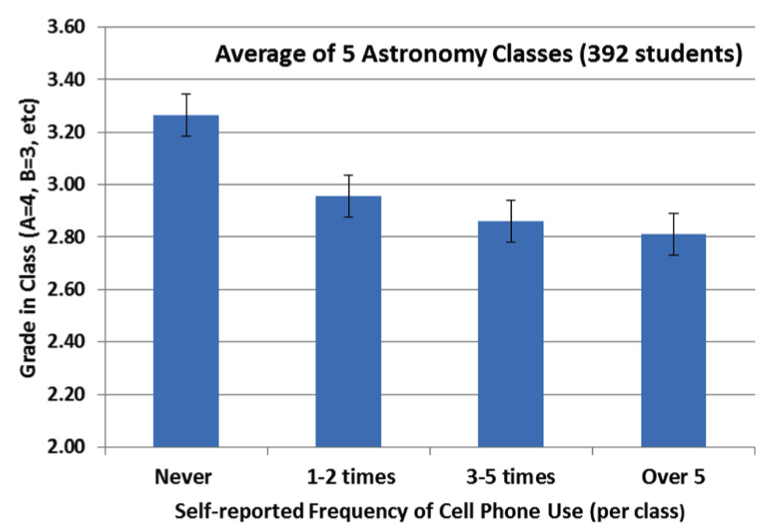
\includegraphics[width=1\textwidth]{cell-phone-data.png}
            \caption{\tiny \shortfullcite{Duncan2012}}
            \end{center}
        \end{figure}
        \end{uncoverenv}

    \end{columns}
    \end{adjustwidth}
\end{frame}
\end{noheadline}

\begin{noheadline}
\begin{frame}[t]
    \frametitle{How does this class work?}

        \vspace{-5mm}
        \begin{itemize}
            \item<1-> Reading quizzes
                \vspace{14mm}
            \item<2-> Clickers
                \vspace{14mm}
            \item<3-> Practic exams
                \vspace{14mm}
            \item<4-> Exams
        \end{itemize}
\end{frame}
\end{noheadline}

\begin{noheadline}
\begin{frame}
    \frametitle{How does this class work?}

    \begin{table}%[htbp]
        \centering
        \begin{tabular}{ l | c c }
            & Old-school & High-structure \\
            Grade & (2002-2003) & (2007-) \\
            \hline
            $< 1.5$ & 17\% & 3.4\% \\
            $\geq 3.5$ & 14.5\% & 24.3\% \\
        \end{tabular}
    \end{table}

\end{frame}
\end{noheadline}

% slide with clicker qs, practice exams, exams

\section{How does science work?}

\begin{noheadline}
\begin{frame}
    \frametitle{Experimental Design Module}

    \begin{columns}

        \column{0.7\linewidth}

        \vspace{-1cm}
        \begin{minipage}[c][\textheight][c]{\linewidth}
        \begin{itemize}
            % \item Interpreting data and designing experiments
            \item Work in groups of 3; middle person is the scribe
            \item Be sure your names are legible
            \item We're here to answer questions
            \item Give the worksheet to any TA before leaving
        \end{itemize}
        \end{minipage}

        \column{0.3\linewidth}

        \vspace{-1cm}
        \begin{figure}
            \begin{center}
            \includegraphics[width=1.25\textwidth]{../images/xkcd-cartoon.png}
            \caption{\tiny \href{https://xkcd.com/242/}{https://xkcd.com/242/}}
            \end{center}
        \end{figure}
    \end{columns}
\end{frame}
\end{noheadline}

\end{document}


